\documentclass[11pt,a4paper,oneside]{article}
\usepackage[UTF8,adobefonts]{ctex}

\usepackage{wrapfig}
\usepackage{indentfirst}
\usepackage{amsmath}
\usepackage{float}
\usepackage{ulem}
\usepackage[top=1in,bottom=1in,left=1.25in,right=1.25in]{geometry}

\usepackage{color}
\usepackage{xcolor}

\usepackage{multirow}

\begin{document}

\begin{figure}[H]
 \centering
  
\includegraphics[width=13cm]{Image/表头.png}
\end{figure}
\begin{center}
\textbf{{\large 实验名称:\uline{          分光仪的调整及其应用       }}}
\end{center}
\section*{一、 实验目的}
\begin{enumerate}
\item 了解分光仪的构造及其主要部件的作用。
\item 学习并掌握分光仪德的调节原理与调节方法。
\item 掌握自准直法和逐次逼近法,巩固消视差调节技术。
\item 学会用干涉法测量三棱镜的顶角。
\end{enumerate}

\section*{二、实验原理}
\subsection*{实验1.分光仪的调整}
\subsubsection*{(1)分光仪的结构}
分光仪的结构因型号不同各有差别,但基本原理是相同的,一般都由底座、刻度读数盘、自准直望远镜、平行光管、载物平台5部分组成。
\begin{description}
\item[三角底座] 在三角底座的中心,装有以垂直的固定轴、望远镜、主刻度圆盘、游标刻度圆盘都可以绕它旋转,这一固定轴右脚分光仪主轴。
\item[刻度圆盘] 圆盘上刻有角度数值的称主刻度盘,其内侧有一游标盘,在游标盘上相对$180^{\circ}$处刻有两个游标。主刻度盘和游标刻度盘都垂直于仪器主轴,并可绕主轴转动。该读数系统由主刻度盘和游标盘组成,沿圆盘一周刻有360个大格,每格$1^{\circ}$,每大格又分成两小格,所以每小格为30'。主刻度盘内侧有一游标盘。主刻度盘可以和望远镜一起转动,游标盘可以和载物台一起转动。游标盘在他的对径方向有两个游标刻度,游标刻度的30小格对应主刻度盘上的29小格,所以这一读数系统的精确度为1’。它的读数原理与游标卡尺完全相同。
\item[载物平台] 载物平台用来放置光学元件,如棱镜光栅等,在其下方有载物台调平螺钉3只,以调节平台倾斜度。用螺钉可调节载物平台的高度,当固紧时平台与游标盘固联。固紧螺钉可使游标盘与主轴固联;拧动螺钉,可使载物台与游标盘一起微动。
\item[自准直望远镜] 

 \begin{figure}[H]
 \centering
  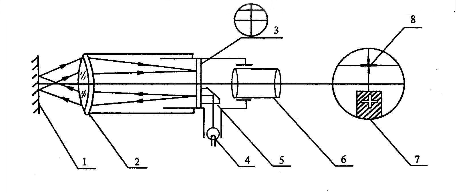
\includegraphics[width=10cm]{Image/自准直望远镜.png}
\end{figure}


自准直望远镜的结构如图所示,它由目镜、全反射镜、叉丝分划板及物镜组成。目镜装在A筒内,全反射棱镜和叉丝分划板装在B筒内,物镜装在C筒顶部,A筒通过手轮可在B筒内前后移动,B筒可在C筒内移动。叉丝分划板上刻有双十字叉丝和透光小十字刻线,并且上叉丝与小十字刻线对称与中心叉丝,全反射棱镜紧贴其上。开启光源S时,光线经全反射棱镜照亮小十字刻线。当小十字刻线平面处在物镜的焦平面上时,从刻线发出的光线经物镜变成平行光。如果有一平面镜将这一平行光反射回来没再经物镜,必成像于焦平面上,于是从目镜中可以看到叉丝和小十字刻线的反射像,并且无视差。如果望远镜光轴垂直于平面反射镜,反射镜将于上叉丝重合。这种调节望远镜光轴使之适于观察平行光的方法成为自准直法,这种望远镜称为自准直望远镜。\\望远镜通过螺钉的固紧可与主刻度盘固联,又可通过螺钉的固紧与主轴固联,此时拧动望远镜微调螺钉,望远镜将连同主刻度盘绕主轴微动。
\item[平行光管] 平行光管与底座固联,靠近仪器主轴的一端装有平行光管的物镜,另一端装有可调节狭缝套管,前后移动套管,是狭缝处在物镜的焦平面上,于是由狭缝产生的光通过物镜后变成平行光。
\end{description}

\subsubsection*{(2)分光仪的调节原理与方法}
分光仪常用于测量入射光与出射光之间的角度,为了能准确测得此角度,必须满足两个条件:
1.入射光与出射光均为平行光;2.入射光与出射光均与刻度盘平面平行。

为此须对分光仪进行调整:使平行光管发出平行光,其光轴垂直于仪器主轴(即平行于刻度盘平面);使望远镜接收平行光,其光轴垂直于仪器主轴;须调整载物平台,使其上旋转的分光元件的光学平面平行于仪器主轴。

\begin{description}
\item[粗调]\hspace*{\fill}\\ 调节水平调节螺钉,使望远镜居于支架中央,并目测调节望远镜俯仰螺钉,使光轴大致与主轴垂直,调节载物平台下方的3只螺钉外伸部分等长,使平台平面大致与主光轴垂直。
\item[调节望远镜]\hspace*{\fill}\\
	\begin{description}
	\item[$\diamondsuit$望远镜调焦于无穷远]\hspace*{\fill}\\
	\textbf{调节要求}: 根据前述自准直原理,当叉丝位于物镜焦平面时,叉丝与小十字刻线的反射像共面,即绿十字与叉丝无视差,此时望远镜只接收平行光,或称望远镜调焦于无穷远。\\ \textbf{调节方法}:在载物平台上放置平面反射镜,构成上图所示的自准直光路。\\开启内藏照明灯泡,照明透光小十字形刻线。调节目镜(转动目镜手轮,筒壁螺纹结构使得目镜筒在叉丝分划板筒内前后移动),改变目镜与叉丝分划板之间的距离,直至看清反射镜沿水平方向的方位,若平面反射镜的镜面在俯仰方向上已大致垂直于望远镜光轴,则在旋转载物台的过程中,总可以在某一位置,通过目镜看到一个绿色十字(可能不太清晰),如看不到则应视情况调节望远镜下方的俯仰螺钉或载物台下方的或螺钉,再一次粗调望远镜光轴大致与平面反射镜的镜面垂直。前后伸缩叉丝分划板套筒B,改变叉丝与物镜之间的距离,直到在目镜中清晰无视差的看到一个明亮的绿色小十字(透光小十字刻线的像)为止。
	\item[$\diamondsuit$调整望远镜光轴与仪器主轴垂直]\hspace*{\fill}\\ 
	\textbf{调整原理}:若望远镜光轴垂直于平面反射镜镜面,且平面镜镜面平行于仪器主轴,则望远镜光轴必垂直于仪器主轴。此时若将载物台绕仪器主轴转180°,使平面镜另一面对准望远镜,望远镜光轴仍将垂直于平面镜。若望远镜光轴开始时垂直于平面镜,但不垂直于仪器主轴,亦即平面镜镜面不平行于主轴,则将平面镜反转180°后,望远镜光轴不再垂直于平面镜镜面。\\
	\textbf{调整方法}:在望远镜调焦于无穷远的基础上,观察绿色小十字,一般它会偏离上叉丝,调节载物台调平螺钉或,使绿色小十字向上叉丝移近1/2的偏离距离,再调节望远镜俯仰调节螺钉,使绿色小十字与上叉丝重合,这时,望远镜光轴与平面镜镜面垂直。将平面镜反转180°,重复调节载物台调平螺钉或,并调节望远镜俯仰调节螺钉,使绿色小十字各自消除1/2与上叉丝的偏离量,再次使望远镜光轴与屏幕镜镜面垂直。如此重复几次,直至平面镜绕主轴旋转180°,绿色小十字始终都落在上叉丝中心为止。每进行一次调节,光轴与主轴垂直状态及平面镜与主轴的平行状态就改善一次。多次调节,逐渐达到完全改善为止,故称为逐次逼近调节。又由于每次各调1/2的偏离量,故又称半调法。
	\item[$\diamondsuit$调整叉丝分划板的纵丝与主轴平行]\hspace*{\fill}\\
	分划板的上叉丝与纵丝是互相垂直的。当纵丝与主轴不平行时,绕主轴转动望远镜,在望远镜视场中,会看到绿色小十字的运动轨迹与上叉丝相交。只要微微转动(不能有前后滑动)叉丝镜筒,达到绿色小十字的运动轨迹与上叉丝重合,叉丝方向就调好了。
	\end{description}
\item[平行光管的调整]\hspace*{\fill}\\
  \begin{description}
    \item[$\diamondsuit$使平行光管产生平行光]\hspace*{\fill}\\ 调整方法:将已调节好的望远镜对准平行光管,拧动狭缝宽度调节手轮,打开狭缝,松开狭缝套筒锁紧螺钉,前后移动狭缝套筒,当在已调焦无穷远的望远镜目镜中无视差的看到边缘清晰的狭缝像时,平行光管即发出平行光。
    \item[$\diamondsuit$调平行光管光轴与仪器主轴垂直]\hspace*{\fill}\\ 调整方法: 旋转望远镜至观察到狭缝像,调整平行光管俯仰调节螺钉,使狭缝像的中点与中心叉丝重合(中心叉丝与狭缝中点都可视为望远镜与平行光管光轴所垂直通过的地方);或将狭缝横放,调平行光管的俯仰调节螺钉至狭缝的固定边与中心叉丝重合。
  \end{description}
\end{description}

至此,分光仪的调整已基本完成,现已满足两个条件:1.入射光与出射光均为平行光;2.入射光与刻度盘平面平行,但出射光还未调至与刻度盘平面平行,这一步与具体的测量内容有关,需结合分光仪的应用来进行。
\subsection*{实验2.三棱镜顶角的测量}
\subsubsection*{(1)三棱镜的调整}
    欲测三棱镜顶角,必须使望远镜的光轴旋转平面垂直于待测顶角A的两光学平面AB面和AC面,即望远镜分别对准AB面和AC面时均应有绿色十字与上叉丝重合。\\
在已调好望远镜的基础上,先用自准直法调AB面与望远镜光轴垂直(即AB面与仪器主轴平行),如不垂直,可调节调平螺钉b或c;再转动载物平台将AC面转向望远镜,此时可且只可调节调平螺钉a使AC面与望远镜光轴垂直,因为调a不会破坏已调好的AB面与望远镜光轴的垂直关系。

\subsubsection*{(2)反射法测三棱镜顶角原理}
     反射法测顶角须使入射平行光经AB、AC面反射后能通过望远镜,而望远镜是绕主轴旋转的,所以AB和AC面的反射平行光必须通过主轴才能进入望远镜。如果主轴中心远离顶角A,AB、AC面的反射光不能通过主轴,从而也就不能通过望远镜;只有如右图所示
     
 \begin{figure}[H]
 \centering
  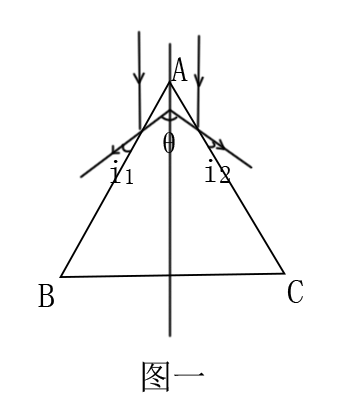
\includegraphics[width=5cm]{Image/反射法测顶角.png}
\end{figure}

     
     顶角A处于主轴中心O附近时,AB、AC面的反射光才能进入望远镜。所以测量顶角时,应尽量将顶角A平移靠主轴中心处。
     旋转载物台至三棱镜顶角A 对准平行光管,使部分平光由 AB 面反射;另一部分
平行光由 AC 面反射。当望远镜在 I 位置观察到 AB 面反射的狭缝像,在 II 位置观察到 AC 面反射的狭缝像时,望远镜转过了角度 $\theta$,所以由图得
\begin{center}
$\theta =A+i_{1}+i_{2}$\\
又因为 $A=i_{1}+i_{2}$\\
故有 $A=\displaystyle\frac{\theta}{2}$
\end{center}
     
\subsection*{实验3.棱镜折射率的测量(最小偏向角法)}

\begin{figure}[H]
 \centering
  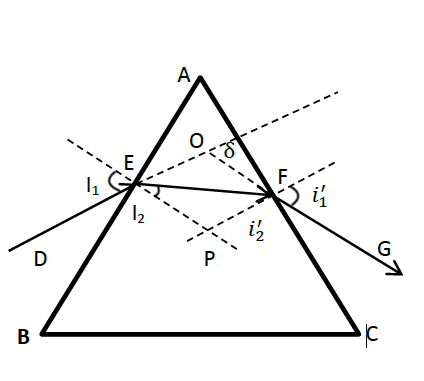
\includegraphics[width=6cm]{Image/最小偏向角法测折射率.png}
\end{figure}

单色平行光束入射到三棱镜AB面,经折射后由AC面出射,出射光线与入射光线的夹角称为偏向角$\delta$。
沿主截面入射的光线DE在界面AB上发生第一次折射,由折射定律有
\begin{center}
$sin{i_1}={n_1}sin{i_2}$
\end{center}
折射光线 EF 入射到界面 AC 上发生第二次折射,同理有
\begin{center}
$sin{i'_2}={n_1}sin{i'_1}$
\end{center}

设三棱镜的顶角为A,由$\bigtriangleup$EOF和$\bigtriangleup$EPF可知

\begin{center}
 $A={i_2}+{i'_2}$\\
 $\delta=({i_1}-{i_2})+({i'_1-i'2})=({i_1}+{i'_1})-({i_2}+{i'_2})=({i_1}+{i'_1})-A$
\end{center}
对顶角一定的棱镜而言,偏向角$\delta$随入射角$i_1$而变;对某个确定的最小值${\delta}_{min}$,称为最小偏
向角。由最小偏向角条件$\displaystyle\frac{d\delta}{d{i_1}}=0$可以证得
\begin{center}
${i_1}={i'_1}$ 或 ${i_2}={i'_2}$
\end{center}
可得
\begin{center}
${i'_2}=\displaystyle\frac{A}{2},{i_{1}}'=\frac{1}{2}(\delta _{min}+A)$
\end{center}
则
\begin{center}
$n_{1}=\displaystyle\frac{\sin\displaystyle\frac{\delta _{min}+A}{2}}{\sin \displaystyle\frac{A}{2}}$
\end{center}

\section*{三、实验仪器}
分光仪、平面反射镜、三棱镜、钠灯及电源。

\section*{四、实验步骤}
\subsection*{实验1.分光仪的调整}
\begin{enumerate}
\item 平面反射镜反射回来的绿色十字与叉丝无视差。
\item 平面镜正、反两面反射回来的绿色十字均与上叉丝重合,且转动平台过程中绿色十字沿上叉丝移动。
\item 狭缝像与叉丝无视差,且中心点与中心叉丝等高。
\end{enumerate}


\subsection*{实验2.三棱镜顶角的测量}
\begin{enumerate}
\item 调整三棱镜\\
将三棱镜放置于载物台上,使待测顶角A靠近中心,并使其一个光学面与载物台上的某根径线平行,用压杆固定好棱镜。将望远镜对准三棱镜某光学平面,调节与另一光学平面平行的在载物台径线下螺钉,使绿色十字与上叉丝重合。同理再调整另一光学平面。
\item 用反射法测棱镜顶角\\
为了准确的测量三棱镜的顶角,除了严格调整分光仪和三棱镜外,尚须准确读取数据和掌握正确的测量方法。
\item 偏心差的消除\\
在分光仪的生产过程中,分光仪的主刻度盘和游标盘不可能完全同心,读数时不可避免地将差生偏差,成为偏心差,这是仪器本身的系统误差。消除系统误差的办法是采用对径读数法。设开始时,左边游标的读数为$\alpha_1$,右边游标的读数为$\beta_1$,当望远镜或载物台转过某一角度后,左边游标的读数为$\alpha_2$,右边游标的读数为$\beta_2$,可以由左边的读数得其转角${\theta_1}={\alpha_2}-{\alpha_1}$,由右边读数得其转角${\theta_2}={\beta_2}-{\beta_1}$,然后取其平均:
\begin{center}
$\theta=\displaystyle\frac{1}{2}({\theta_1}+{\theta_2})=\displaystyle\frac{1}{2}[({\alpha_2}-{\alpha_1})+({\beta_2}-{\beta_1})]$
\end{center}
这就可以消除偏心差,得到准确的结果。
\item 减小主刻度盘刻度不均匀造成的系统误差\\
   如果主刻度盘不均匀,测量时将产生一定的系统误差。为了减少此误差,需在刻度盘不同部位进行多次测量,然后取其平均值。
\item 测量方法\\
每次测量时应改变初始值,即开刻度盘固紧螺钉,单独旋转50◦—60◦,测量次数不少于5次。
注意:推动望远镜的时候应推动望远镜支臂,切勿推动望远镜镜筒,以免破坏望远镜与仪器主轴的垂直关系,造成角度测量的超差。
\end{enumerate}

\subsection*{实验3.棱镜折射率的测量}
\subsubsection*{(1)用最小偏向角法测棱镜折射率}
旋转载物平台,使平行光入射三棱镜的AB面,用望远镜在AC面观察折射光线,之后沿某方向缓慢转动平台,可看到谱线随平台转动向一个方向移动,当移到某个位置时突然向反方向折回,这一转折位置即该谱线的最小偏向位置。测量此位置处谱线与入射光线的夹角,此即最小偏向角${\delta}_{min}$。

\end{document}